% 2019-1-5-data-structure.tex

\documentclass[]{beamer}
% File: preamble.tex
\usepackage{lmodern}

\usepackage{xeCJK}
\usetheme{CambridgeUS} % try Pittsburgh
\usecolortheme{beaver}
\usefonttheme[onlymath]{serif} % try "professionalfonts"

\setbeamertemplate{itemize items}[default]
\setbeamertemplate{enumerate items}[default]

\usepackage{comment}

\usepackage{amsmath, amsfonts, latexsym, mathtools, tabu}
\newcommand{\set}[1]{\{#1\}}
\newcommand{\ps}[1]{\mathcal{P}(#1)}
\usepackage{bm}
\DeclareMathOperator*{\argmin}{\arg\!\min}

\ExplSyntaxOn
\bool_new:N \l__xeCJK_listings_letter_bool
\ExplSyntaxOff
\usepackage{listings}

\definecolor{bgcolor}{rgb}{0.95,0.95,0.92}

\lstdefinestyle{CStyle}{
    language = C,
    basicstyle = \ttfamily\bfseries,
    backgroundcolor = \color{bgcolor},   
    keywordstyle = \color{blue},
    stringstyle = \color{teal},
    commentstyle = \color{cyan},
    breakatwhitespace = false,
    breaklines = true,                 
    mathescape = true,
    escapeinside = ||,
    morekeywords = {procedure, end, foreach, repeat, until},
    showspaces = false,                
    showstringspaces = false,
    showtabs = false,                  
}

% colors
\newcommand{\red}[1]{\textcolor{red}{#1}}
\newcommand{\redoverlay}[2]{\textcolor<#2>{red}{#1}}
\newcommand{\green}[1]{\textcolor{green}{#1}}
\newcommand{\greenoverlay}[2]{\textcolor<#2>{green}{#1}}
\newcommand{\blue}[1]{\textcolor{blue}{#1}}
\newcommand{\blueoverlay}[2]{\textcolor<#2>{blue}{#1}}
\newcommand{\purple}[1]{\textcolor{purple}{#1}}
\newcommand{\cyan}[1]{\textcolor{cyan}{#1}}
\newcommand{\teal}[1]{\textcolor{teal}{#1}}

% colorded box
\newcommand{\rbox}[1]{\red{\boxed{#1}}}
\newcommand{\gbox}[1]{\green{\boxed{#1}}}
\newcommand{\bbox}[1]{\blue{\boxed{#1}}}
\newcommand{\pbox}[1]{\purple{\boxed{#1}}}

\usepackage{pifont}
\usepackage{wasysym}

\newcommand{\cmark}{\green{\ding{51}}}
\newcommand{\xmark}{\red{\ding{55}}}
%%%%%%%%%%%%%%%%%%%%%%%%%%%%%%%%%%%%%%%%%%%%%%%%%%%%%%%%%%%%%%
% for fig without caption: #1: width/size; #2: fig file
\newcommand{\fignocaption}[2]{
  \begin{figure}[htp]
    \centering
      \includegraphics[#1]{#2}
  \end{figure}
}

\usepackage{tikz}
\usetikzlibrary{positioning, mindmap, shadows}

\newcommand{\push}{\texttt{Push}}
\newcommand{\pop}{\texttt{Pop}}

\newcommand{\titletext}{2-3 Counting}

\newcommand{\thankyou}{
  \begin{frame}[noframenumbering]{}
    \fignocaption{width = 0.50\textwidth}{figs/thankyou.png}
  \end{frame}
}

%%%%%%%%%%
\title[\titletext]{\titletext}
\subtitle{}

\author[Hengfeng Wei]{\large 魏恒峰}
\titlegraphic{
\includegraphics[height = 2.0cm]{figs/qrcode-problem-solving-class-2019-1}}
\institute{hfwei@nju.edu.cn}
\date{2019年11月14日}
%%%%%%%%%%
\begin{document}

\maketitle

% % file: overview.tex

%%%%%%%%%%%%%%%
\begin{frame}{}
  \begin{columns}
    \column{0.50\textwidth}
      \fignocaption{width = 0.55\textwidth}{figs/chai}
    \column{0.50\textwidth}
      \pause
      \fignocaption{width = 0.85\textwidth}{figs/xiongan}
  \end{columns}

  \pause
  \vspace{0.50cm}
  \begin{center}
    {\red{\large $Q:$ What is Probability?}} \\[5pt] \pause
    {\violet{\small (Objective? \quad Subjective? \quad Neutral?)}}
  \end{center}
\end{frame}
%%%%%%%%%%%%%%%

%%%%%%%%%%%%%%%
\begin{frame}{}
  \begin{columns}
    \column{0.35\textwidth}
      \fignocaption{width = 0.95\textwidth}{figs/infinity}
    \column{0.30\textwidth}
      \fignocaption{width = 0.70\textwidth}{figs/intuition-told}
    \column{0.35\textwidth}
      \fignocaption{width = 0.90\textwidth}{figs/dice}
  \end{columns}

  \vspace{0.50cm}
  \begin{quote}
    ``\ldots and the many \purple{paradoxes} show clearly that we, as humans, 
    \purple{lack a well grounded intuition} in this matter.''

    \hfill --- {\small ``The Art of Probability'', Richard W. Hamming}
  \end{quote}

  \pause
  \begin{quote}
    ``When called upon to judge probability, people actually judge something else
    and \purple{\bf believe} they have judged probability.''

    \hfill --- {\small ``Thinking, Fast and Slow'', Daniel Kahneman}
  \end{quote}
\end{frame}
%%%%%%%%%%%%%%%

%%%%%%%%%%%%%%%
\begin{frame}{}
  \fignocaption{width = 0.30\textwidth}{figs/Leibniz}

  \pause
  \vspace{0.50cm}
  \begin{quote}
    \centerline{\red{\LARGE Let us calculate [calculemus].}}
  \end{quote}
\end{frame}
%%%%%%%%%%%%%%%

%%%%%%%%%%%%%%%
\begin{frame}{}
  \fignocaption{width = 0.30\textwidth}{figs/open-topics}

  {\large
    \begin{enumerate}[(a)]
      \centering
      \setlength{\itemsep}{6pt}
      \item Monty Hall problem
      \item Boy or Girl paradox
      \item Searching unsorted array
    \end{enumerate}
  }
\end{frame}
%%%%%%%%%%%%%%%

%%%%%%%%%%%%%%%
% \begin{frame}{}
%   \fignocaption{width = 0.45\textwidth}{figs/intuition-vs-calculation}
% 
%   \vspace{0.50cm}
%   \begin{quote}
%     \centerline{\red{\LARGE Intuition {\it vs.} Calculation}}
%   \end{quote}
% \end{frame}
%%%%%%%%%%%%%%%

%%%%%%%%%%%%%%%
\begin{frame}{}
  \begin{center}
    {\LARGE Permutations} \\[1.00cm]

    \pause
    \begin{description}
      \centering
      \item[\Large Generating All Permutations]
	\vspace{0.30cm}
      \item[\Large Stackable/Queueable Permutations]
    \end{description}
  \end{center}
\end{frame}
%%%%%%%%%%%%%%%

%%%%%%%%%%%%%%%
\begin{frame}{}
  \begin{description}
    \centering
    \item[\Large Generating All Permutations]
  \end{description}
\end{frame}
%%%%%%%%%%%%%%%

%%%%%%%%%%%%%%%
\begin{frame}{}
  \begin{exampleblock}{DH 2.9: \# of Permutations}
    Prove that the number of permutations of $n$ (distinct) elements is $n!$.
  \end{exampleblock}

  \pause
  \begin{proof}[\uncover<3->{\red{``坊间''证明}}]
    \begin{description}
      \item[For $a_1$:] We have $n$ choices.
      \item[For $a_2$:] We have $n-1$ choices.
      \item[For $\cdots$:] $\cdots$
    \end{description}
    Then, \# of perms is 
    \[
      n \times (n-1) \times \cdots \times 1 = n!
    \]
  \end{proof}

  \vspace{0.60cm}
  \pause
  \centerline{\Large Prove by mathematical induction on $n$.}
\end{frame}
%%%%%%%%%%%%%%%

%%%%%%%%%%%%%%%
\begin{frame}{}
  \begin{exampleblock}{DH 2.9: \# of Permutations}
    Prove that the number of permutations of $n$ (distinct) elements is $n!$.
  \end{exampleblock}

  \vspace{0.60cm}
  \begin{proof}[Prove by mathematical induction on $n$.]
    \[
      P(n): \text{\# of perms of } n \text{ (distinct) element is } n!
    \]

    \pause
    \begin{description}
      \item[B.S.] $P(1)$
      \item[I.H.] $P(n)$
      \item[I.S.] $P(n) \to P(n+1)$
	\pause
	\[
	  \red{\underbrace{\textcolor{black}{(n + 1)}}_{\text{1st choice}}} 
	  \times \blue{\underbrace{\textcolor{black}{n!}}_{I.H.}} = (n + 1)!
	\]
    \end{description}
  \end{proof}
\end{frame}
%%%%%%%%%%%%%%%

%%%%%%%%%%%%%%%
% \begin{frame}{}
%   \begin{exampleblock}{DH 2.9: \# of Permutations}
%     Prove that the number of permutations of $n$ (distinct) elements is $n!$.
%   \end{exampleblock}
% 
%   \vspace{0.60cm}
%   \begin{columns}
%     \pause
%     \column{0.50\textwidth}
%       \begin{enumerate}[(1)]
% 	\item The ``choosing from'' method:
%       \end{enumerate}
%       \fignocaption{width = 0.70\textwidth}{figs/4-permtree}
%     \pause
%     \column{0.50\textwidth}
%       \begin{enumerate}[(1)]
% 	\setcounter{enumi}{1}
% 	\item The ``inserting into'' method:
%       \end{enumerate}
%       \fignocaption{width = 0.70\textwidth}{figs/4-permtree}
%   \end{columns}
% \end{frame}
%%%%%%%%%%%%%%%

%%%%%%%%%%%%%%%
\begin{frame}[fragile]{}
  \begin{exampleblock}{DH 2.11: Generate All Permutations}
    Design an algorithm which, given a positive integer $n$,
    generates/\blue{prints} all the permutations of $[1 \cdots n]$.
  \end{exampleblock}

  \pause
  \begin{lstlisting}[style = Cstyle]
  void perms (A[], n) {
    if (n == 1)
      print ''A[0]''
    else 
      for (int i = 0; i < n; ++i)
        print ''A[i]''
        perms(A $\gets$ A $\setminus$ A[i], n - 1)
        print ''\n''
  }
  \end{lstlisting}

  \vspace{0.30cm}
  \pause
  \centerline{\texttt{\cyan{\large generate-perms.c}}}
\end{frame}
%%%%%%%%%%%%%%%

%%%%%%%%%%%%%%%
\begin{frame}{}
  \begin{columns}
    \column{0.45\textwidth}
      \fignocaption{width = 0.70\textwidth}{figs/error-crazy}
    \pause
    \column{0.45\textwidth}
      \fignocaption{width = 0.80\textwidth}{figs/recursion-draw}
  \end{columns}
\end{frame}
%%%%%%%%%%%%%%%

%%%%%%%%%%%%%%%
\begin{frame}{}
  \[
    A = [0,1,2,3] \qquad n = 4
  \]
  \fignocaption{width = 0.50\textwidth}{figs/4-permtree}
\end{frame}
%%%%%%%%%%%%%%%

%%%%%%%%%%%%%%%
\begin{frame}[fragile]{}
  \begin{lstlisting}[style = Cstyle]
  void perms (|\purple{prifix}|, A[], n) {
    if (n == 1)
      print ''prifix ++ A[0]''
    else 
      for (int i = 0; i < n; ++i)
        perms(|\purple{prefix $\gets$ prefix ++ A[i]}|, 
            A $\gets$ A $\setminus$ A[i], n - 1)
        print ''\n''
  }
  \end{lstlisting}

  \pause
  \begin{lstlisting}[style = Cstyle]
  perms('''', A, n);
  \end{lstlisting}
\end{frame}
%%%%%%%%%%%%%%%

%%%%%%%%%%%%%%%
\begin{frame}{}
  \begin{columns}
    \column{0.45\textwidth}
      \fignocaption{width = 0.70\textwidth}{figs/taocp-perms}
    \column{0.45\textwidth}
      \fignocaption{width = 0.60\textwidth}{figs/knuth}
  \end{columns}
\end{frame}
%%%%%%%%%%%%%%%

%%%%%%%%%%%%%%%
\begin{frame}{}
  \begin{exampleblock}{DH 2.10: Permutation Checking}
    \begin{itemize}
      \item An integer $n$
      \item An array of integers $P$ of length $n$
    \end{itemize}
    To check whether $P$ is a permutation of $1 \cdots n$?
  \end{exampleblock}

  \begin{columns}[t]
    \pause
    \column{0.45\textwidth}
      \begin{enumerate}
	\item Boolean array $[1 \cdots n]$
      \end{enumerate}

      \pause
      \[
	\blue{\underbrace{O(n)}_{\texttt{time}}} \quad \red{\underbrace{O(n)}_{\text{space}}}
      \]
    \pause
    \column{0.45\textwidth}
      \begin{enumerate}
	\setcounter{enumi}{1}
	\item Sort and then scan
      \end{enumerate}

      \pause
      \[
	\red{\underbrace{O(n \log n)}_{\texttt{time}}} \quad \blue{\underbrace{O(1)}_{\text{space}}}
      \]
  \end{columns}

  \pause
  \begin{columns}
    \column{0.25\textwidth}
      \fignocaption{width = 0.50\textwidth}{figs/question}
    \column{0.20\textwidth}
      \[
	\blue{\underbrace{O(n)}_{\texttt{time}}} \quad \blue{\underbrace{O(1)}_{\text{space}}}
      \]
    \pause
    \column{0.40\textwidth}
      \fignocaption{width = 0.40\textwidth}{figs/baby-dont-know}
  \end{columns}
  % \begin{columns}
  %   \column{0.20\textwidth}
  %   \column{0.60\textwidth}
  %     \begin{enumerate}
  %       \setcounter{enumi}{2}
  %       \centering
  %       \item \begin{itemize}
  %         \item Check $\forall x: x \in [1 \cdots n]$
  %         \item Check for duplication/distinctness
  %       \end{itemize}
  %     \end{enumerate}
  %   \column{0.20\textwidth}
  % \end{columns}
\end{frame}
%%%%%%%%%%%%%%%

%%%%%%%%%%%%%%%
\begin{frame}{}
  \begin{center}
    {\LARGE Stackable Permutations}
  \end{center}
\end{frame}
%%%%%%%%%%%%%%%

% \begin{description}[\texttt{push(X, S)}:]
%   \item[\texttt{read(X)}:] $\texttt{in >> } X$
%   \item[\texttt{print(X)}:] $\texttt{out << } X$
%   \item[\texttt{push(X, S)}:] $S \Leftarrow X$
%   \item[\texttt{pop(X, S)}:] $X \Leftarrow S$
% \end{description}

%%%%%%%%%%%%%%%
\begin{frame}{}
  \begin{definition}[Stackable Permutations]
    \uncover<2->{
      \[
	\fbox{$\texttt{out} = (a_1, \cdots, a_n) \blue{\xleftarrow[\;X \;=\; 0\;]{\;S \;=\; \emptyset\;}} \texttt{in} = (1, \cdots, n)$}
      \]
    }

    \fig{width = 0.65\textwidth}{figs/stack-perm-x}
  \end{definition}
\end{frame}
%%%%%%%%%%%%%%%

%%%%%%%%%%%%%%%
\begin{frame}{}
  \begin{definition}[Stackable Permutations]
    \fig{width = 0.50\textwidth}{figs/stack-perm-x}
  \end{definition}

  \vspace{0.20cm}
  \pause
  \begin{center}
    \red{$Q_2:$} Using \cyan{only} ``\texttt{read, print, push, pop}''?
  \end{center}

  \pause
  \[
    a == X  \pause \qquad \texttt{top}(S) \pause \qquad \red{a > X \; (a < X)}
  \]
\end{frame}
%%%%%%%%%%%%%%%

%%%%%%%%%%%%%%%
\begin{frame}{}
  \fig{width = 0.50\textwidth}{figs/stack-perm-x}

  \begin{center}
    \red{We can assume that $X$ is always blank.}
  \end{center}

  \pause
  \begin{proof}
    \begin{center}
      What are the possible operations following \texttt{read(X)}/\texttt{pop(X, S)}? \\
    \end{center}
  \end{proof}
\end{frame}
%%%%%%%%%%%%%%%

%%%%%%%%%%%%%%%
\begin{frame}{}
  \begin{exampleblock}{DH 2.12: Stackable Permutations}
    \begin{enumerate}[(a)]
      \item Show that the following permutations \emph{\blue{are}} stackable:
	\begin{enumerate}[(i)]
	  \item $(3, 2, 1)$
	  \item \textcolor{purple}{$(3, 4, 2, 1)$}
	  \item $(3, 5, 7, 6, 8, 4, 9, 2, 10, 1)$
	\end{enumerate}
    \end{enumerate}
  \end{exampleblock}

  \pause
  \vspace{0.50cm}
  \fig{width = 0.40\textwidth}{figs/no-choice}
\end{frame}
%%%%%%%%%%%%%%%

%%%%%%%%%%%%%%%
\begin{frame}[fragile]{}
  \begin{exampleblock}{DH 2.13: Stackable Permutations Checking Algorithm}
    To check whether a given permutation can be obtained by a stack.

    \centerline{\texttt{read} \quad \texttt{print} \quad \texttt{push} \quad \texttt{pop} \quad \red{\texttt{is-empty}}}
  \end{exampleblock}


  \begin{lstlisting}[style = Cstyle]
              X = 0    S = $\emptyset$    in != EOF
  \end{lstlisting}

  \begin{columns}
    \pause
    \column{0.45\textwidth}
      \begin{lstlisting}[style = Cstyle]
foreach 'a' in out:
  if (! is-empty(S) 
      && 'a' == top(S))
    pop(S, X)
    print(X)
      \end{lstlisting}
    \pause
    \column{0.45\textwidth}
      \begin{lstlisting}[style = Cstyle]
  else // T.B.C
    while (in != EOF)
      read(X)
      if (X == 'a')
        print(X)
        break
      else
        push(X, S)
    if (in == EOF)
      ERR
      \end{lstlisting}
  \end{columns}
\end{frame}
%%%%%%%%%%%%%%%

%%%%%%%%%%%%%%%
\begin{frame}{}
  \begin{exampleblock}{DH 2.12: Stackable Permutations}
    \begin{enumerate}[(a)]
      \setcounter{enumi}{1}
    \item \red{\bf Prove} that the following permutations are \emph{\blue{not}} stackable:
	\begin{enumerate}[(i)]
	  \item $(3, 1, 2)$
	  \item $(4, 5, 3, 7, 2, 1, 6)$
	\end{enumerate}
    \end{enumerate}
  \end{exampleblock}

  \uncover<2->{
    \[
      (\red{3}, \red{1}, \red{2})
    \]

    \[
      (4, 5, 3, \red{7}, \red{2}, 1, \red{6})
    \]
  }

  \uncover<3->{
    \[
      \fbox{$\texttt{out} = \cdots a_i \cdots a_j \cdots a_k: i < j < k \land a_j < a_k < a_i$}
    \]
  }

  \uncover<4->{
    \[
      312\text{-Pattern}
    \]
  }
\end{frame}
%%%%%%%%%%%%%%%

%%%%%%%%%%%%%%%
\begin{frame}[fragile]{}
  \begin{theorem}[Stackable Permutations]
    A permutation $(a_1, \cdots, a_n)$ is stackable $\iff$ it is not the case that
    \[
      312\text{\it -Pattern}: \fbox{$\texttt{\it out} = \cdots a_i \cdots a_j \cdots a_k: i < j < k \land a_j < a_k < a_i$}
    \]
  \end{theorem}

  \vspace{0.30cm}
  \pause
  \begin{proof}
    \fig{width = 0.40\textwidth}{figs/no-proof}
  \end{proof}

  % \pause
  % \begin{proof}
  %   \begin{columns}
  %     \column{0.45\textwidth}
  %       \[
  %         \text{stackable} \Longrightarrow \nexists \;312\text{-Pattern} 
  %       \]
  %       \pause
  %       \[
  %         \blue{312\text{-Pattern} \Longrightarrow \text{non-stackable}}
  %       \]
  %       \pause
  %       \[
  %         \red{\forall \;\text{algorithms}}
  %       \]
  %     \column{0.45\textwidth}
  %       \pause
  %       \[
  %         \blue{\nexists \;312\text{-Pattern} \Longrightarrow \text{stackable}}
  %       \]
  %       \pause
  %       \[
  %         \red{\exists \;\text{algorithm}}
  %       \]
  %   \end{columns}
  % \end{proof}
\end{frame}
%%%%%%%%%%%%%%%

%%%%%%%%%%%%%%%
% \begin{frame}{}
%   \begin{theorem}[Stackable Permutations]
%     A permutation $(a_1, \cdots, a_n)$ is stackable \blue{(on the model $S$)} $\iff$ it is not the case that
%     \[
%       312\text{\it -Pattern}: \fbox{$\texttt{\it out} = \cdots a_i \cdots a_j \cdots a_k: i < j < k \land a_j < a_k < a_i$}
%     \]
%   \end{theorem}
% 
%   \vspace{0.30cm}
%   \begin{proof}[$312\text{-Pattern} \Longrightarrow \text{non-stackable}$]
%     \begin{description}[$a_j < a_k < a_i$:]
%       \item[$a_j < a_k < a_i$:] When $a_i$ is poped, $a_j$ and $a_k$ are on the stack.
%       \item[$j < k$:] $a_j$ is above $a_k$ on the stack.
%       \item[$a_j < a_k$:] Contradiction.
%     \end{description}
%   \end{proof}
% \end{frame}
%%%%%%%%%%%%%%%

%%%%%%%%%%%%%%%
% \begin{frame}[fragile]{}
%   \begin{theorem}[Stackable Permutations]
%     A permutation $(a_1, \cdots, a_n)$ is stackable \blue{(on the model $S$)} $\iff$ it is not the case that
%     \[
%       312\text{\it -Pattern}: \fbox{$\texttt{\it out} = \cdots a_i \cdots a_j \cdots a_k: i < j < k \land a_j < a_k < a_i$}
%     \]
%   \end{theorem}
% 
%   \vspace{0.30cm}
%   \begin{proof}[$\nexists \;312\text{-Pattern} \Longrightarrow \text{stackable}$]
%     \centerline{According to our algorithm and by contradiction.}
% 
%     \[
%       a_j \notin \texttt{in} \land a_j \;!\!= \texttt{top}(S) \implies \exists k > j: a_k > a_j
%     \]
% 
%     \[
%       a_j, a_k \implies \exists i < j (< k): a_j < a_k < a_i
%     \]
%   \end{proof}
% \end{frame}
%%%%%%%%%%%%%%%

%%%%%%%%%%%%%%%
\begin{frame}{}
  \begin{exampleblock}{DH 2.12: Stackable Permutations}
    \begin{enumerate}[(a)]
      \setcounter{enumi}{2}
      \item How many permutations of $A_4$ \red{\emph{cannot}} be obtained by a stack?
    \end{enumerate}
  \end{exampleblock}

  \begin{align*}
    &(1, \redoverlay{4}{2-}, \redoverlay{2}{2-}, \redoverlay{3}{2-}), (2, 4, 1, 3), (3, 1, 2, 4), 
    (\redoverlay{3}{2-}, \redoverlay{1}{2-}, 4, \redoverlay{2}{2-}), (3, 4, 1, 2) \\
    &(4, 1, 2, 3), (4, 1, 3, 2), (\redoverlay{4}{2-}, 2, \redoverlay{1}{2-}, \redoverlay{3}{2-}), (4, 2, 3, 1), (4, 3, 1, 2)
  \end{align*}

  \vspace{0.60cm}
  \uncover<3->{\centerline{\red{$Q:$} What about $A_n$?}}
\end{frame}
%%%%%%%%%%%%%%%

%%%%%%%%%%%%%%%
\begin{frame}{}
  \begin{columns}[b]
    \column{0.50\textwidth}
      \fig{width = 0.90\textwidth}{figs/stack-perm-x}
    \pause
    \column{0.50\textwidth}
      \fig{width = 0.90\textwidth}{figs/stack-perm}
  \end{columns}

  \pause
  \vspace{1.00cm}

  \begin{center}
    {\red{$Q:$} Are $S+X$ and $S$ are \red{\bf equivalent}?} \\[15pt]

    \pause
    {\blue{Producing the same set of permutations.}}
  \end{center}
\end{frame}
%%%%%%%%%%%%%%%

%%%%%%%%%%%%%%%
\begin{frame}{}
  \begin{columns}[b]
    \column{0.50\textwidth}
      \fig{width = 0.90\textwidth}{figs/stack-perm-x}
    \column{0.50\textwidth}
      \fig{width = 0.90\textwidth}{figs/stack-perm}
  \end{columns}

  \vspace{0.40cm}
  \pause
  \begin{proof}[\large By simulations.]
    \begin{columns}[t]
      \pause
      \column{0.45\textwidth}
        Simulate $S$ by $S + X$:
	\begin{itemize}
	  \item \texttt{Push}
	  \item \texttt{Pop}
	\end{itemize}
      \pause
      \column{0.45\textwidth}
        Simulate $S + X$ by $S$:
	\pause
	\[
	  \text{By iterative transformations.}
	\]
    \end{columns}
  \end{proof}
\end{frame}
%%%%%%%%%%%%%%%

%%%%%%%%%%%%%%%
% \begin{frame}{}
%   \fig{width = 0.50\textwidth}{figs/stack-perm}
% 
%   \[
%     (1, 2, 3): \push{}\;\; \pop{}\;\; \push{}\;\; \pop{}\;\; \push{}\;\; \pop{}\;\;
%   \]
% 
%   \[
%     (3, 2, 1): \push{}\;\;\push{}\;\;\push{}\;\;\pop{}\;\;\pop{}\;\;\pop{}\;\;
%   \]
%   % \[
%   %   (3, 2, 5, 6, 1, 4): \push{}\;\;\push{}\;\;\push{}\;\;\pop{}\;\;\pop{}\;\;\push{}\;\;\push{}\;\;\pop{}\;\;\push{}\;\;\pop{}\;\;\pop{}\;\;\pop{}\;\;
%   % \]
% \end{frame}
%%%%%%%%%%%%%%%

%%%%%%%%%%%%%%%
\begin{frame}{}
  \begin{exampleblock}{DH 2.12: Stackable Permutations}
    How many permutations of $\set{1 \cdots n}$ are stackable \blue{on the model $S$}?
  \end{exampleblock}

  \fig{width = 0.50\textwidth}{figs/stack-perm}

  \pause
  \centerline{\red{$Q:$} How many \blue{\emph{admissible}} operation sequences of \purple{``\texttt{Push}''} and \purple{``\texttt{Pop}''}?}
\end{frame}
%%%%%%%%%%%%%%%

%%%%%%%%%%%%%%%
\begin{frame}{}
  \begin{definition}[Admissible Operation Sequences]
    An operation sequence of \purple{``\texttt{Push}''} and \purple{``\texttt{Pop}''} is \blue{\it admissible} if and only if
    \begin{enumerate}[(i)]
      \pause
      \item $\# \text{ of ``\texttt{Push}''} = n \qquad \# \text{ of ``\texttt{Pop}''} = n$
      \pause
      \item $\forall \text{ prefix}: (\# \text{ of ``\texttt{Pop}''}) \le (\# \text{ of ``\texttt{Push}''})$
    \end{enumerate}
  \end{definition}

  \vspace{0.50cm}
  \pause
  \begin{center}
    \red{\fbox{\# of stackable perms $=$ \# of admissible operation sequences}}
  \end{center}
\end{frame}
%%%%%%%%%%%%%%%

%%%%%%%%%%%%%%%
\begin{frame}{}
  \begin{theorem}
    Different admissible operation sequences correspond to different permutations.
  \end{theorem}

  \vspace{0.30cm}
  \pause
  \begin{proof}
    \begin{align*}
      &\push{}\; \;\push{}\; \;\push{}\; \;\pop{}\; \;\pop{}\; \;\red{\push{}} \cdots \\
      &\push{}\; \;\push{}\; \;\push{}\; \;\pop{}\; \;\pop{}\; \;\red{\pop{}} \cdots \\
    \end{align*}
  \end{proof}
\end{frame}
%%%%%%%%%%%%%%%

%%%%%%%%%%%%%%%
\begin{frame}{}
  \begin{theorem}
    The number of admissible operation sequences of \texttt{\it \purple{``Push''}} and \texttt{\it \purple{``Pop''}} is ${2n \choose n} - {2n \choose n-1}$.
  \end{theorem}

  \pause
  \begin{proof}[Proof: The Reflection Method]
    \[
      \push{}: \;\rightarrow \qquad \pop{}: \;\uparrow
    \]

    \begin{columns}
      \pause
      \column{0.50\textwidth}
	% \fig{width = 0.90\textwidth}{figs/grid-path}
	\begin{center}
	  \resizebox{0.80\textwidth}{!}{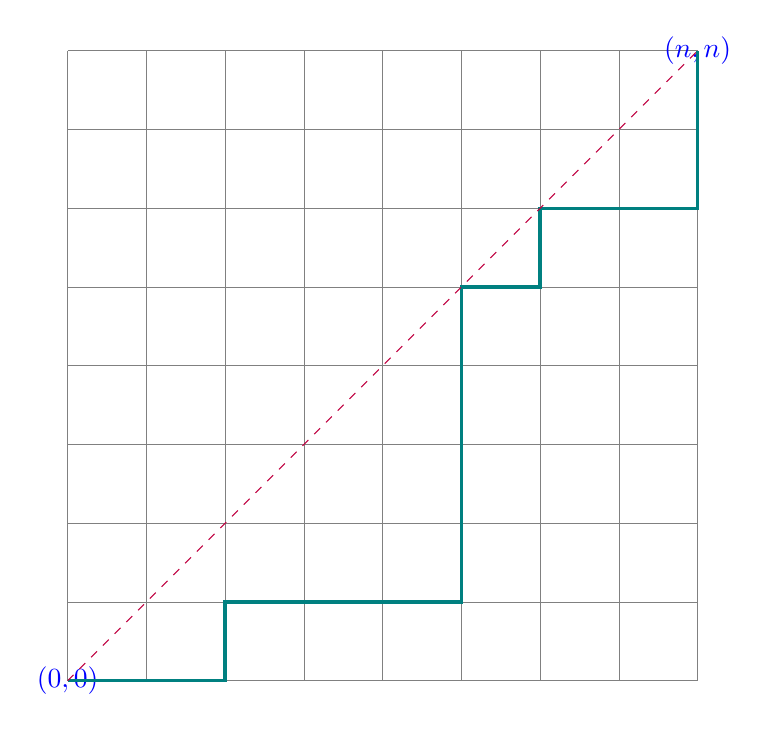
\begin{tikzpicture}
  \draw[help lines] (0,0) grid (8,8);

  \node (00) [blue] {$(0,0)$};
  \node (nn) [blue] at (8,8) {$(n,n)$};

  \pause
  \draw[teal, very thick] (0,0) -- (1,0) -- (2,0) 
    -- (2,1) -- (3,1) -- (4,1) -- (5,1) 
    -- (5,2) -- (5,3) -- (5,4) -- (5,5)
    -- (6,5) -- (6,6)
    -- (7,6) -- (8,6)
    -- (8,7) -- (8,8);

  \pause
  \draw[purple, dashed] (00.center) to (nn.center);
\end{tikzpicture}
}
	\end{center}
      \column{0.50\textwidth}
	\uncover<6->{
	  \[
	    \blue{\underbrace{\textcolor{black}{{2n \choose n}}}_{\text{all}}} 
	    - \red{\underbrace{\textcolor{black}{{2n \choose n-1}}}_{\text{inadmissible}}}
	  \]
	}
    \end{columns}
  \end{proof}
\end{frame}
%%%%%%%%%%%%%%%

%%%%%%%%%%%%%%%
\begin{frame}{}
  \begin{center}
    \resizebox{0.60\textwidth}{!}{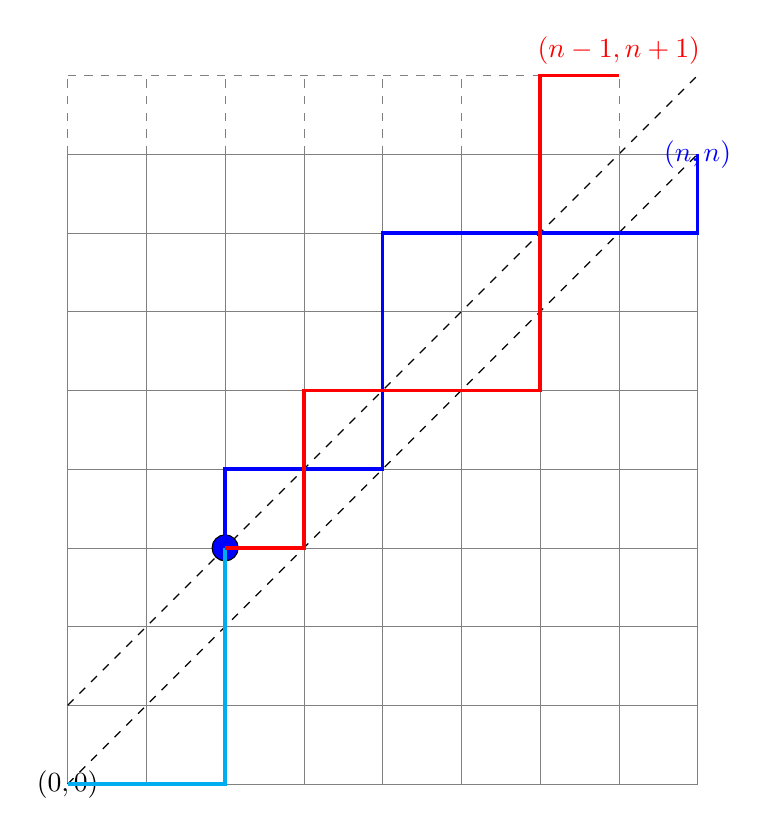
\begin{tikzpicture}
  \draw[help lines] (0,0) grid (8,8);

  \node (00) [] {$(0,0)$};
  \node (01) [] at (0,1) {};
  \node (nn) [blue] at (8,8) {$(n,n)$};

  \draw [dashed] (0,0) to (8,8);

  \pause
  \draw[very thick] (0,0) -- (1,0) -- (2,0) --
	(2,1) -- (2,2) -- (2,3);
  \draw[very thick] (2,3) -- (2,4) --
	(3,4) -- (4,4) --
	(4,5) -- (4,6) -- (4,7) --
	(5,7) -- (6,7) -- (7,7) -- (8,7) --
	(8,8);

  \pause
  \node (nn1) [] at (8,9) {};
  \draw [dashed] (0,1) to (8,9);

  \pause
  \node () [circle, draw, fill = blue] at (2,3) {};

  \pause
  \draw[very thick, cyan] (0,0) -- (1,0) -- (2,0) --
	(2,1) -- (2,2) -- (2,3);
  \draw[very thick, blue] (2,3) -- (2,4) --
	(3,4) -- (4,4) --
	(4,5) -- (4,6) -- (4,7) --
	(5,7) -- (6,7) -- (7,7) -- (8,7) --
	(8,8);

  \pause
  \draw[help lines, dashed] (0,8) grid (7,9);
  \draw[very thick, red] 
	(2,3) -- (3,3) --
	(3,4) -- (3,5) --
	(4,5) -- (5,5) -- (6,5) --
	(6,6) -- (6,7) -- (6,8) -- (6,9) --
	(7,9) node[above] () {$(n-1, n+1)$};
\end{tikzpicture}}
  \end{center}
\end{frame}
%%%%%%%%%%%%%%%

%%%%%%%%%%%%%%%
\begin{frame}{}
  \begin{center}
    \resizebox{0.60\textwidth}{!}{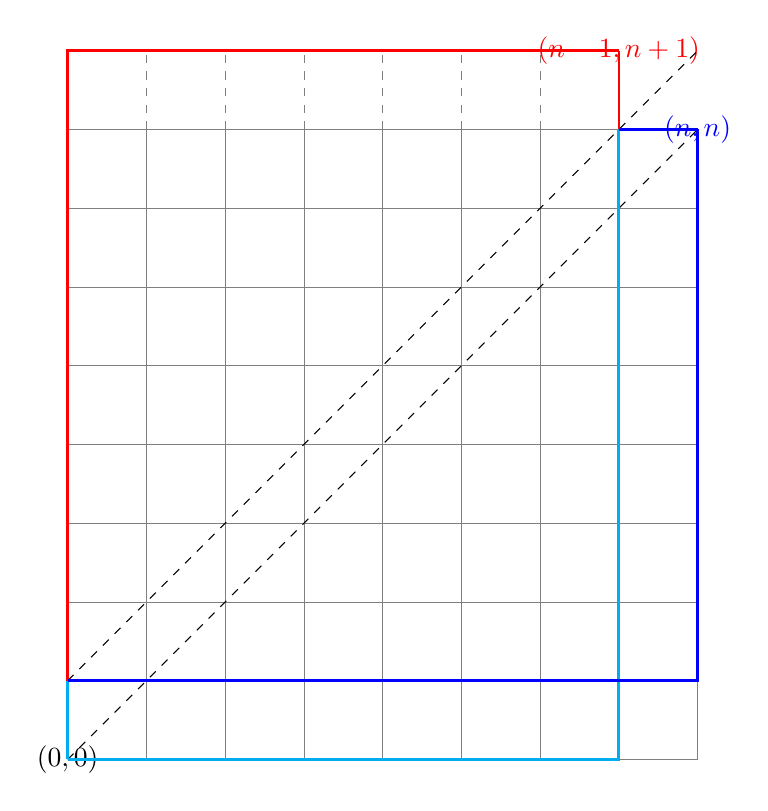
\begin{tikzpicture}
  \draw[help lines] (0,0) grid (8,8);
  \draw[help lines, dashed] (0,8) grid (7,9);

  \node (00) [] {$(0,0)$};
  \node (01) [] at (0,1) {};
  \node (nn) [blue] at (8,8) {$(n,n)$};
  \node (nn1) [] at (8,9) {};
  \node (n1n1) [red] at (7,9) {$(n-1, n+1)$};

  \draw [dashed] (0,0) to (8,8);
  \draw [dashed] (0,1) to (8,9);

  \uncover<2-3>{
    \draw[very thick, cyan] (0,0) -- (7,0) -- (7,8);
  \draw[thick, red] (7,8) -- (7,9);
  }
  \uncover<3>{
    \draw[very thick, blue] (7,8) -- (8,8);
  }

  \uncover<4-5>{
    \draw[very thick, cyan] (0,0) -- (0,1);
    \draw[very thick, red] (0,1) -- (0,9) -- (7,9);
  }
  \uncover<5>{
    \draw[very thick, blue] (0,1) -- (8,1) -- (8,8);
  }
\end{tikzpicture}
}
  \end{center}
\end{frame}
%%%%%%%%%%%%%%%

%%%%%%%%%%%%%%%
\begin{frame}{}
  \centerline{\Large \href{https://en.wikipedia.org/wiki/Catalan\_number}{Catalan Number}}

  \[
    (3,2,1): ((())) \qquad (1,2,3): ()()()
  \]
\end{frame}
%%%%%%%%%%%%%%%

%%%%%%%%%%%%%%%
\begin{frame}{}
  \begin{center}
    {\Large For more about ``Stackable Permutations'' {\large (Section $2.2.1$)}}
  \end{center}

  \vspace{0.30cm}
  \begin{columns}
    \column{0.45\textwidth}
      \fig{width = 0.60\textwidth}{figs/taocp1}
    \column{0.45\textwidth}
      \fig{width = 0.50\textwidth}{figs/knuth}
  \end{columns}
\end{frame}
%%%%%%%%%%%%%%%

\thankyou{}
\end{document}
%%%%%%%%%%